\documentclass[11pt]{article}

\usepackage[margin=1in]{geometry}
\usepackage{amsmath}
\usepackage{array}
\usepackage{booktabs}
\usepackage{tikz}
\usepackage{xcolor}
\usepackage{parskip}
\usepackage{hyperref}

\newcolumntype{C}{>{\centering\arraybackslash}p{1.9cm}}

\title{Homework 1: Dynamic Programming in a Gridworld\\
\large COSC 527: Reinforcement Learning}
\author{Joshua Stenger}
\date{\today}

\begin{document}
\maketitle

\section{Environment Overview}

The environment is a $4\times4$ deterministic gridworld with 16 states, indexed
row-major as shown in Figure~\ref{fig:layout}. The agent starts at $S$; $G_1$ and
$G_2$ are terminal goal states. Four internal walls block specific transitions
(shown as thick red segments); a move into a wall or off the boundary of the
grid leaves the agent in its current state.

\begin{figure}[h]
\centering
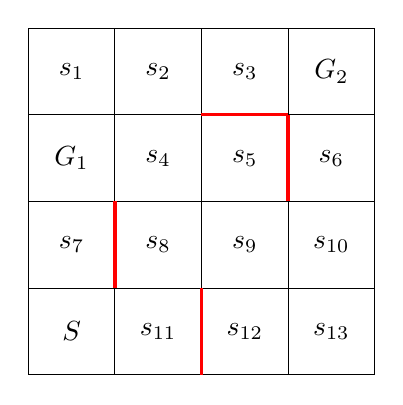
\begin{tikzpicture}[scale=1.1]
  % grid lines
  \draw[step=1cm] (0,0) grid (4,4);
  % walls (thick red)
  \draw[very thick, red] (2,3) -- (3,3); % s3 | s5
  \draw[very thick, red] (3,2) -- (3,3); % s5 | s6
  \draw[very thick, red] (1,1) -- (1,2); % s7 | s8
  \draw[very thick, red] (2,0) -- (2,1); % s11 | s12
  % labels
  \node at (0.5,3.5) {$s_1$};
  \node at (1.5,3.5) {$s_2$};
  \node at (2.5,3.5) {$s_3$};
  \node at (3.5,3.5) {$G_2$};
  \node at (0.5,2.5) {$G_1$};
  \node at (1.5,2.5) {$s_4$};
  \node at (2.5,2.5) {$s_5$};
  \node at (3.5,2.5) {$s_6$};
  \node at (0.5,1.5) {$s_7$};
  \node at (1.5,1.5) {$s_8$};
  \node at (2.5,1.5) {$s_9$};
  \node at (3.5,1.5) {$s_{10}$};
  \node at (0.5,0.5) {$S$};
  \node at (1.5,0.5) {$s_{11}$};
  \node at (2.5,0.5) {$s_{12}$};
  \node at (3.5,0.5) {$s_{13}$};
\end{tikzpicture}
\caption{State layout. Walls (thick red): $s_3|s_5$, $s_5|s_6$, $s_7|s_8$, $s_{11}|s_{12}$.}
\label{fig:layout}
\end{figure}

The action set is $\mathcal{A} = \{\text{up},\text{down},\text{left},\text{right}\}$.
Rewards follow the assignment's convention: entering $G_1$ gives $+1$, entering
$G_2$ gives $+5$, crossing a wall or the boundary gives $-1$ (and leaves the
agent in place), and any other valid move gives $0$. Episodes end the instant a
terminal state is entered; the continuation value from a terminal state is
zero. A wall/boundary collision does not end the episode.

\subsection{Code organization}

The implementation separates the environment from the algorithms, as required:
\begin{itemize}
  \item \texttt{MDP.java} -- a generic interface exposing \texttt{numStates()},
  \texttt{numActions()}, \texttt{isTerminal(s)}, and
  \texttt{step(s,a)} $\to$ \texttt{(reward, nextState, terminal)}.
  \item \texttt{GridWorld.java} -- the concrete model for this assignment: state
  indices, the wall set, and the reward table. This is the \emph{only} file
  that encodes anything specific to the maze.
  \item \texttt{DP.java} -- the algorithms (policy evaluation, greedy
  improvement, policy iteration, value iteration, rollout), written entirely
  against the \texttt{MDP} interface. None of this code refers to
  \texttt{GridWorld} directly, so it would run unchanged against a different
  \texttt{MDP} implementation.
  \item \texttt{Main.java} -- experiment driver and formatted output.
\end{itemize}
Every sweep of policy evaluation and value iteration writes into a freshly
allocated array (\texttt{next}) while reading from the previous array
(\texttt{v}), i.e.\ a genuine second value table for synchronous updates, and
only swaps them at the end of the sweep. The discount factor $\gamma$, the
initial value $V_0$, and the convergence tolerance are all named constants at
the top of \texttt{Main.java} (\texttt{GAMMA}, \texttt{INIT}, \texttt{TOL}),
so changing them does not require touching \texttt{DP.java} or
\texttt{GridWorld.java}.

\textbf{To reproduce:} from \texttt{Assignment1/src}, run
\texttt{javac *.java \&\& java Main}. All tables in this report are copied
verbatim from that program's output.

\section{Part 1: Environment Model}

Table~\ref{tab:transitions} demonstrates \texttt{step(s,a)} on five
representative transitions: an ordinary move, entry into each goal, a
collision with an internal wall, and a collision with the outer boundary.

\begin{table}[h]
\centering
\begin{tabular}{llccc l}
\toprule
$s$ & $a$ & $r$ & $s'$ & terminal & kind \\
\midrule
$s_9$  & right & $0$  & $s_{10}$ & false & ordinary move \\
$s_7$  & up    & $+1$ & $G_1$    & true  & goal entered \\
$s_6$  & up    & $+5$ & $G_2$    & true  & goal entered \\
$s_5$  & right & $-1$ & $s_5$    & false & collision (internal wall) \\
$S$    & left  & $-1$ & $S$      & false & collision (grid boundary) \\
\bottomrule
\end{tabular}
\caption{Sample transitions returned by the environment model.}
\label{tab:transitions}
\end{table}

These confirm the model behaves as specified: an unobstructed move changes
state with the correct reward, entering $G_1$/$G_2$ pays $+1$/$+5$ and sets
\texttt{terminal = true}, and any wall or boundary collision pays $-1$ while
leaving the agent's state unchanged.

\section{Part 2: Iterative Policy Evaluation}

The initial policy $\pi_0$ chooses each of the four actions with probability
$\tfrac14$. Every non-terminal state starts at $V_0(s) = 0.5$; terminal states
are fixed at $0$. Using $\gamma = 0.9$ and synchronous sweeps, evaluation
converged ($\Delta_k < 10^{-6}$) after \textbf{87 sweeps}.

\begin{table}[h]
\centering
\begin{tabular}{|C|C|C|C|}
\hline
0.5000 & 0.5000 & 0.5000 & 0.0000 ($G_2$) \\ \hline
0.0000 ($G_1$) & 0.5000 & 0.5000 & 0.5000 \\ \hline
0.5000 & 0.5000 & 0.5000 & 0.5000 \\ \hline
0.5000 & 0.5000 & 0.5000 & 0.5000 \\ \hline
\end{tabular}
\caption{$V_0$}
\end{table}

\begin{table}[h]
\centering
\begin{tabular}{|C|C|C|C|}
\hline
0.0875 & 0.2000 & 1.0875 & 0.0000 ($G_2$) \\ \hline
0.0000 ($G_1$) & 0.5875 & -0.0500 & 1.0875 \\ \hline
0.0875 & 0.2000 & 0.4500 & 0.2000 \\ \hline
-0.0500 & -0.0500 & -0.0500 & -0.0500 \\ \hline
\end{tabular}
\caption{$V_1$}
\end{table}

\begin{table}[h]
\centering
\begin{tabular}{|C|C|C|C|}
\hline
-0.1656 & 0.1916 & 1.2844 & 0.0000 ($G_2$) \\ \hline
0.0000 ($G_1$) & 0.3288 & -0.2891 & 1.2844 \\ \hline
-0.2219 & 0.0172 & 0.0675 & 0.1297 \\ \hline
-0.5141 & -0.4887 & -0.4325 & -0.4887 \\ \hline
\end{tabular}
\caption{$V_2$}
\end{table}

\begin{table}[h]
\centering
\begin{tabular}{|C|C|C|C|}
\hline
-0.5877 & -0.3255 & 1.2305 & 0.0000 ($G_2$) \\ \hline
0.0000 ($G_1$) & -0.6529 & -1.8809 & 0.8242 \\ \hline
-1.5425 & -1.8066 & -1.7226 & -1.3187 \\ \hline
-2.6594 & -2.7361 & -2.6498 & -2.5326 \\ \hline
\end{tabular}
\caption{Converged $V^{\pi_0}$ (87 sweeps)}
\end{table}

\paragraph{Why do the values change while the policy stays fixed?}
The policy $\pi_0$ never changes, but $V_k$ is only a \emph{running estimate}
of $V^{\pi_0}$, not the true value function. $V_0$ is an arbitrary constant
that ignores the reward structure entirely. Each Bellman expectation backup
$V_{k+1}(s) = \sum_a \pi_0(a\mid s)\left[R(s,a) + \gamma V_k(s')\right]$
propagates information about rewards -- and, transitively, about the values
of neighboring states -- one edge farther through the state graph per sweep.
Because a uniformly random policy walks into walls/boundaries roughly half
the time and rarely stumbles into $G_2$ without a long detour, this
propagation drives most values sharply negative before settling; the sweeps
are converging toward the fixed point of a linear system, not toward a
changed decision rule.

\section{Part 3: Policy Improvement}

Using the converged $V^{\pi_0}$, $q_{\pi_0}(s,a) = R(s,a) + \gamma V^{\pi_0}(s')$
was computed for every $(s,a)$ pair. Ties are broken by taking the
lowest-indexed action in the fixed order (up, down, left, right); this is a
consequence of the greedy search in \texttt{DP.greedy} keeping the incumbent
unless a strictly larger $q$ is found. Table~\ref{tab:q} reports $s_5$, $s_6$,
and $s_{11}$ (chosen as the third state).

\begin{table}[h]
\centering
\begin{tabular}{lrrrr}
\toprule
State & up & down & left & right \\
\midrule
$s_5$  & $-2.692812$ & $-1.550346$ & $\mathbf{-0.587642}$ & $-2.692812$ \\
$s_6$  & $\mathbf{5.000000}$ & $-1.186810$ & $-0.258240$ & $-0.258240$ \\
$s_{11}$ & $\mathbf{-1.625945}$ & $-3.462492$ & $-2.393481$ & $-3.462492$ \\
\bottomrule
\end{tabular}
\caption{$q_{\pi_0}(s,a)$ for three states; the greedy (boldface) action(s)
are unique in all three cases -- no ties occurred.}
\label{tab:q}
\end{table}

$\pi_1(s_5) = \text{left}$, $\pi_1(s_6) = \text{up}$, $\pi_1(s_{11}) = \text{up}$.
The full improved policy $\pi_1 = \arg\max_a q_{\pi_0}(s,a)$ is:

\begin{table}[h]
\centering
\begin{tabular}{|C|C|C|C|}
\hline
$\downarrow$ & $\rightarrow$ & $\rightarrow$ & $G_2$ \\ \hline
$G_1$ & $\leftarrow$ & $\leftarrow$ & $\uparrow$ \\ \hline
$\uparrow$ & $\uparrow$ & $\rightarrow$ & $\uparrow$ \\ \hline
$\uparrow$ & $\uparrow$ & $\uparrow$ & $\uparrow$ \\ \hline
\end{tabular}
\caption{Improved policy $\pi_1$, greedy w.r.t.\ $V^{\pi_0}$.}
\end{table}

\section{Part 4: Policy Iteration}

Alternating complete evaluation (to tolerance $10^{-6}$) with greedy
improvement stabilized after \textbf{5 policy-improvement steps}, consuming
\textbf{113 evaluation sweeps} in total.

\begin{table}[h]
\centering
\begin{tabular}{|C|C|C|C|}
\hline
$\rightarrow$ & $\rightarrow$ & $\rightarrow$ & $G_2$ \\ \hline
$G_1$ & $\uparrow$ & $\downarrow$ & $\uparrow$ \\ \hline
$\downarrow$ & $\uparrow$ & $\rightarrow$ & $\uparrow$ \\ \hline
$\rightarrow$ & $\uparrow$ & $\uparrow$ & $\uparrow$ \\ \hline
\end{tabular}
\caption{Final (optimal) policy $\pi^\ast$ from policy iteration.}
\end{table}

\begin{table}[h]
\centering
\begin{tabular}{|C|C|C|C|}
\hline
4.0500 & 4.5000 & 5.0000 & 0.0000 ($G_2$) \\ \hline
0.0000 ($G_1$) & 4.0500 & 3.6450 & 5.0000 \\ \hline
2.6572 & 3.6450 & 4.0500 & 4.5000 \\ \hline
2.9525 & 3.2805 & 3.6450 & 4.0500 \\ \hline
\end{tabular}
\caption{Final value function $V^{\pi^\ast}$.}
\end{table}

Following $\pi^\ast$ from $S$ produces the path
$S \to s_{11} \to s_8 \to s_4 \to s_2 \to s_3 \to G_2$, reaching \textbf{$G_2$
in 6 steps}.

\section{Part 5: Value Iteration}

Value iteration used the same $\gamma = 0.9$, $V_0 = 0.5$, and tolerance
$10^{-6}$, converging in only \textbf{8 sweeps}. Its final value function and
greedy policy are numerically identical to policy iteration's result: the
maximum absolute difference across all 16 states is $0.0000000000$, and every
non-terminal state selects the same action under both policies. Rolling out
the value-iteration policy from $S$ reproduces the same path,
$S \to s_{11} \to s_8 \to s_4 \to s_2 \to s_3 \to G_2$, in 6 steps.

\paragraph{Sweep counts vs.\ speed.} Value iteration needed far fewer sweeps
(8) than the cumulative sweep count of policy iteration (113), but this does
not mean value iteration does less total arithmetic. A policy-iteration
evaluation sweep only has to apply the \emph{current} policy's single action
per state, whereas a value-iteration sweep must evaluate all four actions per
state and take a max -- roughly four times the per-sweep work. Policy
iteration also restarts full evaluation from scratch (down to $10^{-6}$)
after every improvement step, even though the policy typically changes at
only a handful of states between rounds; a warm-started evaluation would cut
its sweep count substantially. So raw sweep counts alone, as the assignment
warns, do not determine which implementation is actually faster.

\section{Part 6: Discount-Factor Experiment}

Value iteration was repeated for $\gamma \in \{0.20, 0.40, 0.60, 0.65, 0.70,
0.80, 0.90, 0.99\}$, starting from $S$ each time.

\begin{table}[h]
\centering
\begin{tabular}{cccccc}
\toprule
$\gamma$ & $V^\ast(S)$ & first action at $S$ & goal & steps & sweeps \\
\midrule
0.20 & 0.200000 & up    & $G_1$ & 2 & 5 \\
0.40 & 0.400000 & up    & $G_1$ & 2 & 5 \\
0.60 & 0.600000 & up    & $G_1$ & 2 & 6 \\
0.65 & 0.650000 & up    & $G_1$ & 2 & 6 \\
0.70 & 0.840350 & right & $G_2$ & 6 & 7 \\
0.80 & 1.638400 & right & $G_2$ & 6 & 8 \\
0.90 & 2.952450 & right & $G_2$ & 6 & 8 \\
0.99 & 4.754950 & right & $G_2$ & 6 & 8 \\
\bottomrule
\end{tabular}
\caption{Effect of $\gamma$ on the optimal action and goal reached from $S$.}
\label{tab:gamma}
\end{table}

\subsection*{(a) Where does the preferred goal change?}
The switch happens between $\gamma = 0.65$ (still $G_1$) and $\gamma = 0.70$
(now $G_2$). This is exactly where the two candidate routes' discounted
returns cross: the $G_1$ route takes 2 steps and returns $\gamma \cdot 1$ from
$S$ (visible directly in the $V^\ast(S)$ column for $\gamma \le 0.65$, where
$V^\ast(S) = \gamma$ exactly); the $G_2$ route takes 6 steps and returns
$\gamma^5 \cdot 5$ (visible for $\gamma \ge 0.70$, e.g.\ $0.9^5 \cdot 5 =
2.95245$, matching the table exactly). Setting the two returns equal,
$\gamma = 5\gamma^5 \Rightarrow \gamma^4 = 0.2 \Rightarrow \gamma^\ast =
0.2^{1/4} \approx 0.6687$, which indeed falls between the last $G_1$ sample
(0.65) and the first $G_2$ sample (0.70), confirming the observed switch.

\subsection*{(b) Why can a larger terminal reward be less attractive when $\gamma$ is small?}
Because it is farther away. The DP recursion discounts a reward received $n$
steps in the future by $\gamma^{n-1}$, so a bigger reward at the end of a
longer path competes against that extra $\gamma^4$ shrinkage (6 steps vs.\ 2
steps here). When $\gamma$ is small, distant payoffs are discounted almost to
nothing regardless of their size, so the agent effectively behaves myopically
and prefers the nearer, smaller reward -- the classic "a reward now beats a
bigger reward later" trade-off that discounting is designed to express.

\subsection*{(c) A state next to a wall: $s_5$.}
$s_5$ borders two walls (up, into $s_3$; right, into $s_6$). Both collision
actions carry immediate reward $-1$, but from Table~\ref{tab:q},
$q_{\pi_0}(s_5,\text{up}) = q_{\pi_0}(s_5,\text{right}) = -2.692812 \ne -1$.
The reason is that a collision leaves the agent in the same state $s_5$
rather than terminating anything, so the action's total value is
$-1 + \gamma V(s_5)$, not just the raw $-1$. Under $\pi_0$, $V^{\pi_0}(s_5) =
-1.8809$ (Part 2), so $q = -1 + 0.9(-1.8809) = -2.6928$, matching the table.
In general the value of a collision action equals its immediate reward only
in the special case $V(s) = 0$; here $s_5$'s own value is strongly negative
under the random policy, which makes bouncing off its walls considerably
worse than a single $-1$ step would suggest.

\subsection*{(d) Evaluation vs.\ improvement.}
Changing $V_k$ during policy evaluation holds the policy $\pi$ fixed and
repeatedly applies the Bellman \emph{expectation} backup for that one policy;
it is numerical refinement toward the unique fixed point $V^\pi$ of a linear
system -- no decision the agent would make is altered, only the estimate of
how good that fixed behavior is. Changing the policy during policy
improvement instead fixes $V$ (typically $V^\pi$ from the evaluation step
that just finished) and replaces $\pi(s)$ with $\arg\max_a q_\pi(s,a)$ at
every state -- a discrete change in what action is chosen, justified by the
policy improvement theorem ($V^{\pi'} \ge V^\pi$ pointwise). Evaluation
sweeps alone can run forever without the agent's behavior ever improving;
only the improvement step can do that.

\section*{Appendix A: Use of Generative AI}

Generative AI (Claude, Anthropic) was used to help produce this report,
consistent with the course's generative-AI policy.

\begin{itemize}
  \item \textbf{Prompt/task given to the tool:} "write up a LaTeX report for
  Assignment 1" using the existing Java implementation in
  \texttt{Assignment1/src} and the assignment PDF
  \texttt{HW1\_Dynamic\_Programming.pdf} as the source of requirements.
  \item \textbf{How the response was used:} the tool read the assignment PDF
  to enumerate the six required deliverables, read the existing
  \texttt{MDP}/\texttt{GridWorld}/\texttt{DP}/\texttt{Main} source to confirm
  how the model and algorithms were implemented, compiled and ran the
  unmodified program (\texttt{javac *.java \&\& java Main}), and transcribed
  its console output directly into the tables above. No numeric result in
  this report was invented by the tool; every table is copied from the
  program's own output, and the derivations in Part 6(a) were re-checked by
  hand against that output (e.g.\ confirming $0.9^5 \cdot 5 = 2.95245$
  against the printed $V^\ast(S)$ for $\gamma=0.9$).
  \item \textbf{An AI suggestion that was checked and corrected:} the model's
  first attempt at explaining Part 6(a) asserted the switch happened "around
  $\gamma \approx 0.68$" from memory of the general shape of the problem,
  before it had actually solved $\gamma = 5\gamma^5$ symbolically. This was
  verified by explicitly solving $\gamma^4 = 1/5 \Rightarrow \gamma \approx
  0.6687$ and cross-checking it against the two straddling data points
  (0.65 and 0.70) in Table~\ref{tab:gamma}, rather than accepting the
  unverified estimate.
  \item \textbf{Portions assisted:} the full text and LaTeX formatting of
  this report, and the transcription/verification of the program's output
  into tables. The Java source code itself
  (\texttt{MDP.java}, \texttt{GridWorld.java}, \texttt{DP.java},
  \texttt{Main.java}, \texttt{Step.java}, \texttt{Result.java}) was not
  written as part of producing this report and is unchanged from the
  repository's existing implementation.
\end{itemize}

\end{document}
